\documentclass[useAMS,usenatbib]{emulateapj}
\usepackage{graphicx}
\usepackage{epsfig}
\usepackage{natbib}
%\usepackage{lscape}
%\usepackage{subfigure}
\usepackage{verbatim}
%\usepackage{multicolumn}
\usepackage{amssymb,amsmath}
%\mathindent 5.mm

%\newcommand{\aj}{AJ}
%\newcommand{\apj}{ApJ}
%\newcommand{\apjl}{ApJ Letters}
%\newcommand{\apjs}{ApJ Supp.}
%\newcommand{\mnras}{MNRAS}
%\newcommand{\nat}{Nature}
\usepackage{color}

\newcommand{\prate}{\dot\chi}
\DeclareMathVersion{bold}
\newcommand{\erf}{\mathrm{erf}\mathnormal{}}
\newcommand{\tobs}{t_{\rm obs}} \newcommand{\ton}{t_{\rm on}}
\newcommand{\src}{BCG\,2261}
\newcommand{\eg}{e.\,g.}
\newcommand{\msun}{M_{\odot}}
\newcommand{\rcusp}{$r_\gamma$}
\newcommand{\fixme}[1]{{\color{red} #1 }}

\shorttitle{The black hole in Abell 2261}
\shortauthors{Everyone et al.}

%\date{}
%\hyphenation{ }

\begin{document} 

\title{Assessing Gravitational Recoil in the Abell 2261 Brightest Cluster Galaxy}

%\author{S. Djorgovski\altaffilmark{1,2,3} and Ivan R. King\altaffilmark{1}}
%\affil{Astronomy Department, University of California, Berkeley, CA 94720}

\author{Everyone}
\affil{From all the important places}
%^&\author{S. Burke-Spolaor\altaffilmark{1,2}\thanks{Email: sarah.spolaor@csiro.au}}
%^&\affil{NRAO}

%\maketitle

\begin{abstract}
%We report a study of the brightest cluster galaxy in Abell 2261, which is host to the largest-known galaxy core of cusp radius 3.2\,kpc. We have collected HST and VLA data on this object to study the history and nature of its compact radio jet and its central knots. We find that the radio jet is a relic, with an age of $>$$10^6$\,y. We weigh three possibilities for the history of this radio jet in the context of standard active nucleus lifecycles and in the context of merger processes, concluding that XXXXX. We find that at least two of the knots in \src\ are dwarf galaxies being cannibalized by their massive host. However, the two remaining knots remain viable contenders for hosting the ``missing'' supermassive black hole in this galaxy.
\fixme{This paper reports VLA and HST observations of the brightest cluster galaxy in Abell 2261, which is host to the largest known galaxy core (cusp radius 3.2~kpc).  Such a large core is hypothesized to result from the ''scouring'' action associated with the merger of two supermassive black holes (SMBHs), and our observations were designed to identify the resulting merged SMBH.  We find a compact radio jet, with a likely age in excess of $10^6$~yr and potentially associated with one of the previously-known optical knots, and we conclude that two of the optical knots are likely to be dwarf galaxies in the process of being cannibalized by their host galaxy.  We are not able to identify conclusively any remnant SMBH, with the two other optical knots remaining as candidate ''shrouds'' of stars that might be captured by the remnant SMBH following the merger.  [Brief description of what future observations might have a hope of finding the remnant SMBH or concluding that it has been ejected from the galaxy entirely.]}
%http://adsabs.harvard.edu/abs/2016ApJ...829...81B
\end{abstract}

\keywords{...}



\section{Is the Large Core in A2261-BCG Due To an Ejected Black Hole?}

It is now understood that supermassive back holes are not only common
to the centers of galaxies, but have masses closely tied to the
properties of their hosts \citep{mag,msig,ferraresemerrittmsig}.  A galaxy and its black hole
are formed and evolve together, each influencing the other.

The existence of ``cores'' in the central distribution of stars
in luminous elliptical galaxies are hypothesized to be an example of this.
Cores are regions over which the central stellar density distribution breaks
and shallows out as the center of the galaxy is approached,
in contrast to the steep envelope density profile of the surrounding galaxy.
They were first seen in high resolution images of elliptical
galaxies obtained from the ground \citep{l85, k85},
and studied extensively in {\it Hubble Space Telescope} images
\citet{f94,l95,laine03,l05}.

\citet{begelman80} suggested that a binary black hole would create a core during
the merger of two galaxies as stars were ejected from the center of
the newly created system as the binary slowly hardened.
N-body simulations have demonstrated this
phenomenon directly \citep{ebisuzaki91, makino97, milomerritt01}.
\citet{faber97} offered strong observational support for this scenario,
showing that the most luminous elliptical galaxies nearly always have cores,
and are correlated with slow-rotation and ``boxy'' isophotes in these systems,
while less-luminous or rapidly rotating ellipticals rarely have cores.
Core formation is thus a natural end-point of
``dry mergers'' of two progenitor galaxies.

But if there is strong circumstantial evidence that cores are made by the
hardening of a supermassive black hole binary,
direct observational proof for the existence of such binaries is still lacking.
Other phenomena that come into play during the evolution of the binary
may leave their own imprint on the central structure
of the hosting galaxies, however, and thus strengthen the case if observed.
If the initial formation of the binary is followed by a subsequent merger,
a three-body interaction with a third black hole newly introduced
into the central potential may cause all holes to be ejected from the core.
Apart from this, the terminal hardening of the binary and the subsequent
merging of the two holes into one may generate a strong jet of gravitational
radiation that ejects the merged product from the core as well \citep{recoilfx1}.
In either case the sudden removal of the black hole mass would
cause the core to rebound and expand in size.  If the black hole is
not ejected from the galaxy, but remains on a radial orbit that
returns it to the center, energy exchange with the stars in the core
via dynamical friction may also enlarge the core well beyond its initial
size as produced by the hardening of the binary \citep{bk04, m04}.

\citet{postman12} called attention to the exceptionally large core
in the galaxy A2261-BCG as a candidate site where the central black
hole may have been ejected from the center of system.
The stellar surface brightness distribution has a cusp radius (the
radius at which the local logarithmic slope of the profile is $-1/2$)
$r_\gamma=3.2$~kpc, twice as big as that in the BCG NGC 6166,
the largest core in the \citet{lauer07} compilation,
which incorporates the extensive {\it HST} imaging survey of 
nearby BCGs of \citet{laine03}.

\citet{postman12} further show that the A2261-BCG has a completely flat or
even slightly depressed brightness profile interior to the core.
Most cores generally have singular, if shallow, cusps interior to
the cusp radius \citep{l95,l05}.  A small number of galaxies
have cores with centrally {\it decreasing} brightness profiles,
but they are rare \citep{l02,l05}.

The completely flat core of A2261-BCG strongly resembles
the large cores formed by ejection of the central black hole \citep{gm}.
The core of A2261-BCG is also slightly displaced from the photo-center of the
surrounding galaxy, suggesting a relatively recent dynamical 
disturbance, while the rest of the galaxy shows no evidence for recent
interaction.  Lastly, there are four compact low-luminosity
``knots'' in close proximity to the core.  The ejected black hole
is predicted to carry a tightly bound compact ``cloak" of stars
with it, potentially similar to these knots \citet{m09}.




%The brightest cluster galaxy in Abell 2261 (hereafter \src) is a galaxy of extremes; at \mbox{$\sigma=387\pm16\,{\rm km\,s^{-1}}$}, it has a stellar velocity dispersion among the highest values observed in all galaxies. It also is one of the most luminous BCGs known, with a total absolute magnitude --24.70 in the $V$ band. Furthermore, \src\ was recently revealed to have a core with two abnormal features: its core radius, \rcusp, is 3.2\,kpc (0.89$''$), more than two times the largest core known; and its surface brightness profile is flat, consistent with scouring by a supermassive black hole pair with a total mass of $\sim$$10^{10}\,\msun$ \citep{postman12}. Postman et al.\ hypothesized that the most likely scenario for this system is that its supermassive binary underwent a gravitational recoil following coalescence, thus further scouring the core. Their analysis of this system indicated several interesting features, including four compact, non-central optical knots within the core region, and a displacement of the central galactic core within its envelope at 0.7$"$ to the northeast. The knots were not identifiable from previously available data, but it remained a hypothesis that one or several of them contain a supermassive black hole. If so, this would lend strong support for a post-coalescence recoil scenario for \src.

Here we present a detailed study of \src\ with the Hubble Space Telescope (HST) and the Jansky Very Large Array (VLA). These observations were aimed primarily at exploring the simple question: \emph{Where is the gigantic black hole that should reside in this galaxy?} \fixme{Outline sections here}

%It is also possible that the pair has already coalesced, and either resides centrally in the system
%Previous studies have demonstrated that the size and shape of galaxy cores likely correlate with the merger history and mass of the central black hole in the galaxy. 




\begin{table*}
\centering
\caption{VLA Imaging Results \fixme{Beam/source P.A.'s and numbers need to be triple-checked.}}
\begin{tabular}{cccccccccc}
\hline
        & $f_{\rm center}$ &  {\bf $\sigma$} & {\bf Peak}        & {\bf Int.} & {\bf Beam size} & {\bf Beam} &{\bf Source Size} & {\bf Source} & {\bf Linear}\\
{\bf Band} & {\bf (GHz)} & {\bf ($\mu$Jy)}& {\bf ($\mu$Jy)} & {\bf ($\mu$Jy)} & {\bf (mas)}& {\bf P.A. (deg)} &{\bf (mas)} & {\bf P.A. (deg)} & {\bf extent (kpc)}\\
\hline
% These are flux/beam size numbers from **POOR** fits.
C & 5.873 & 2.1 & $132.4\pm6.8$ & $483\pm31$ &$530\times360$& 68.0 & 950$\pm$$70\times470$$\pm$60& $135\pm5$&3.45\\
X & 9.937 & 1.2 & $23.4\pm1.9$   & $158\pm14$ & $340\times220$ & 72.0& 840$\pm$$80\times490$$\pm$60& $126\pm9$&3.05\\
% Where did I get the below numbers? Is it from kvis or something?!?
%C & 5.873 & 2.1 & 142.1 & 10.1 &$530\times360$& 68.0 & 950$\pm$$70\times470$$\pm$60& $135\pm5$\\
%X & 9.937 & 1.2 & 27.3   &  2.63 &  & xxx& xxx&  xxx\\
\hline
\end{tabular}\label{table:radio}
\vspace{1mm}
\end{table*}

\section{New Data on \src}\label{sec:data}
\subsection{Very Large Array}\label{sec:VLAdata}
As reported by \citet{postman12}, \src\ was detected by the FIRST survey \citep{FIRST} as an unresolved 1.4\,GHz radio source with a flux of 3.4\,mJy, 1.6$''$ west of the galaxy's position; this is just under a factor of two of the galaxy core radius. 
We thus collected wide-band continuum data from the VLA to obtain:
\begin{itemize}
\item Accurate reference frame ties to the available \mbox{SUBARU} optical image to determine whether the offset position was genuine;
\item A resolved image of the core to assess morphological history; and
\item An estimate of the jet age through a rough spectral aging assessment \citep[\eg][]{carilli+91}.
\end{itemize}

Data was collected under project code VLA/15A-061 in A-configuration in two frequency ranges. The first was 3.976--8.024\,GHz (C-band, $f_{\rm avg}=5.873$\,GHz after flagging, hereafter ``6\,GHz''), which provided a resolution of $0.3''$ resolution. The second was 7.976--11.896\,GHz (X-band, $f_{\rm avg}=9.937$\,GHz, hereafter ``10\,GHz''), which provided $0.2''$ imaging resolution. 
%These frequencies both have resolutions well-matched to the available Hubble Space Telescope images. 
Both frequency set-ups used standard 2\,MHz channel widths and 2\,s sampling. Standard primary calibrator 3C286 was used for flux density and bandpass calibration, and source J1735+3616 was used as a phase calibrator. To gain sufficient detection sensitivity, observations were performed in two epochs and then concatenated to create a single data set per frequency band. Given the extended emission in the source, we do not expect intrinsic variability.

The 6\,GHz observations were performed on 11 July 2015, and 13 July 2013, giving a total of 6.27\,h on-source time.
At 10\,GHz, the observations were made on 25 June 2015 and 27 June 2015; 6.70\,hours were spent on-source at this frequency. We utilized the standard VLA pipelines to calibrate the data, and performed manual flagging and imaging with the {\tt CASA} software package. Table\,\ref{table:radio} provides the resulting image noise, measurement, and beam parameters.

%We imaged he VLA observations 
%^&We employed a full bandwidth of 2.048\,GHz, broken into 16 spectral windows, each containing 64 channels of 2\,MHz width. The centre frequency is 8.936\,GHz. The full 27-antenna array was online for our observations. The observations of \src\ were centred at right ascension $\alpha=$~17:22:27.18, declination $\delta=$~+32:07:57.30; this was the position noted by \citep{postman12} to be the galaxy centre.
%The observations and data reduction followed standard VLA phase-reference experiment procedures. 3C286 was used as a primary flux and bandpass calibrator, and standard VLA calibrator J1735+3616 was observed every 10\,min for $\sim$50\,s to provide phase-reference calibration. The total time on \src\ was !!!N!!! minutes. Standard calibration and imaging were performed using the {\sc casa} software package.

%Image properties are given in Table\,\ref{table:radio}. In Figure \ref{fig:contopt}, we show the 
%, and several views of the resulting images are shown in 
%Figs.\,\ref{fig:contopt}--\ref{fig:last}.


\subsection{Hubble Space Telescope}\label{sec:HSTdata}

%\section{HST Observations}
\subsection{Imaging}

Photometry and morphology of the A2261 BCG and the 4 knots seen near its core are based on HST data obtained as part of the Cluster Lensing And Supernova survey with Hubble (CLASH) multi-cycle treasury program. The imaging observations were performed between 09-March-2011 and 21-May-2011 in 16 broadband filters from 2250 \AA\ to $1.6~\mu{\rm m}$. The center of Abell 2261 was observed for a total of 20 orbits. Complete details of the HST imaging data acquisition and reduction are given in \cite{clash}.

\subsection{Spectroscopy}

Spectra of knots 1, 2, and 3 were obtained using the Space Telescope Imaging Spectrograph (STIS) from 31-July-2015 to 01-Aug-2015. We used the G750L grating and the $52'' \times 0.5''$ slit. The initial pointing was centered on the brightest knot (knot 3 at R.A. $=17^h\ 22^m\ 27.14^s$ and Dec. $=+32^o\ 07'\ 57.59''$ (J2000)). The observations were performed with an ORIENT angle of $130.5^{\circ}$ allowing all three knots to be observed simultaneously (see Figure~\ref{stis_orient}). We integrated for a total of 8 orbits (total exposure time of 19,100 seconds) and acquired 16 exposures over that time. The 8 orbit integration sequence was executed as two visits, with 300 second acquisition exposures done at the start of orbits \#1 and \#5 to ensure precise slit alignment. Four small pointing shifts (each $0.2''$ in size and parallel to the long dimension of the slit) were made over the course of 4 orbits to allow for rejection of hot/bad pixels in the dispersion direction. The same shifts were repeated for the second set of 4 orbits. 

\begin{figure}[!t]
\begin{center}
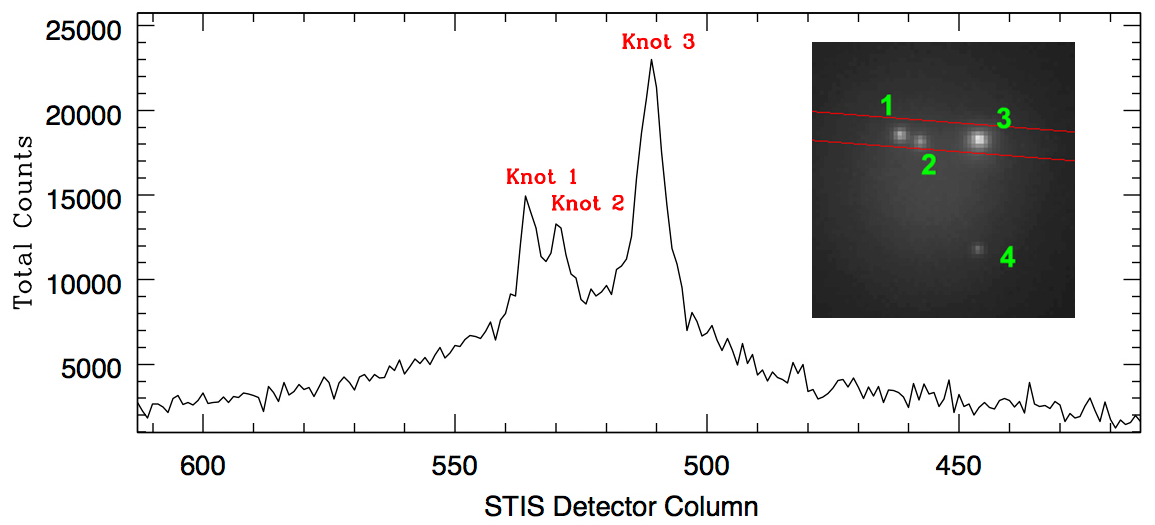
\includegraphics[width=1.0\columnwidth]{figs/compact_STIS_slit_geometry_with_profile.jpg}
\end{center}
\caption{The summed spatial profile across 200 rows of the STIS detector demonstrating the acquisition of photons from all three targeted knots. The inset image shows the STIS $52'' \times 0.5''$ slit orientation as red lines, superposed on an HST F775W image of the core of \src. The four knots in the A2261 BCG core are numbered by their IDs from \cite{postman12}. The ORIENT angle for the STIS observations was $130.5^{\circ}$ corresponding to a position angle on the sky of  $85.5^{\circ}$. This orientation allowed spectra for knots 1, 2, and 3 to be obtained simultaneously. In this image, North is up and West is to the right.}
\label{stis_orient}
\vspace{1mm}
\end{figure}

The STIS data were reduced by performing subtraction of variable herring-bone pattern noise, bias correction and pixel-based charge transfer inefficiency (CTI) correction on the raw science datasets, then running the remainder of the {\tt calstis} processing steps to produce the final CTI-corrected 2D flat-fielded images. The removal of the herring-bone pattern noise, a known issue with STIS since it resumed operations in 2001 using its Side-2 electronics, was done using the procedures outlined in \cite{jansen}. The 2D flat-fielded images were then shifted along the spatial axis using the Pyraf task {\tt sshift} to remove the offsets from the dithers done between each orbit. The individual images were co-added using the {\tt ocrreject} routine, which is designed to detect and remove cosmic rays in STIS CCD data as well as co-add input images. The benefits of using {\tt ocrreject} to combine the data task are twofold: (1) an error array is produced which is proportional to the square-root of the output science image, but smaller by a factor that depends upon the square-root of the number of non-rejected input values used to compute the science pixel values and (2) it allowed us to use all 16 exposures to ensure robust CR-rejection. The final 1D spectrum for each knot was extracted using the {\tt x1d} routine which also applies the STIS flux and wavelength calibrations to produce a co-added 1D spectrum in F$_\lambda$ units of erg s$^{-1}$ cm$^{-2}$ \AA$^{-1}$. The wavelength range of the extracted 1D spectra runs from 5257 \AA\ to 10249 \AA, with a dispersion of 4.87 \AA\ per pixel.

The average signal-to-noise ratio (SNR) per resolution element (resel) in the 1000 \AA\ wide range centered on the redshifted NaD doublet feature (centered at 7207 \AA\ at the  redshift of $z=0.223$ for A2261) for the extracted spectra from knots 1, 2, and 3 is 8.6, 7.7, and 10.7, respectively. The predicted per resel SNR estimates in our original HST proposal were about a factor of 1.8 higher than the achieved values. The large difference between the observed and predicted SNR is primarily due to the significant number of pixels lost to cosmic ray contamination (even with 16 independent exposures) and, to a lesser degree, by residual noise left after the CTI and pattern noise corrections are applied. However, without applying those corrections the observed SNR would have been much worse.

%\subsection{Other data}\label{sec:OTHERdata}
%\fixme{ !!! This section might be worthwhile if we end up using a lot of the previous data from e.g. Postman+12 !!!}

%^&\begin{table*}
%^&\begin{centering}
%^&  \caption{ }\label{table:}
%^&\begin{tabular}{ccccccc}
%^&\hline\hline {\bf } & \multicolumn{2}{c}{\bf Radio centroid} & \multicolumn{2}{c}{\bf Optical offset} & & \\
%^&{\bf Source} & {\bf $\alpha$} & {\bf $\delta$} & {\bf $\Delta\alpha$} & {\bf$\Delta\delta$} & column? & column?\\
%^&%\hline
%^&\src        &  &  &  &  &  & \\
%^&src1       &  &  &  &  &  & \\
%^&src2       &  &  &  &  &  & \\
%^&\hline
%^&(Average) & --- & --- & & & --- & ---\\
%^&\hline\hline
%^&\end{tabular}
%^&\end{centering}
%^&\end{table*}

\section{Velocity Dispersion Measurements}

We fitted the extracted, normalized STIS spectra and estimate the stellar velocity dispersion in the knots.  We used pPXF, the penalized pixel fitting code due to \citet{2004PASP..116..138C}.  
For each knot spectrum we logarithmically rebinned in wavelength so that it matched that of the MILES library spectra \citep{2010MNRAS.404.1639V} we used for our fitting.  To match the spectra, we convolved the higher resolution spectra with a gaussian with variance equal to the difference in variance of our observations and the template spectra.  
We tried various schemes of binning the spectrum but found they made little difference to our final results.  Thus the effective resolution is $250\,\mathrm{km\,s^{-1}}$.    We similarly tried a variety of multiplicative and additive polynomials to account for any residual continuum shape but there was no significant improvement to the fits.  Because of the low signal-to-noise ratio of our data, we fit only the first two moments (velocity, $V$, and velocity dispersion, $\sigma$) of the line-of-sight velocity distribution relative to the recessional velocity of A2261.

A major concern for our fits to data of low signal-to-noise ratio is spurious effects of template mismatch.  In order to take this into consideration we took two precautions.  First, we used the full MILES library.  Second, we ran a series of bootstrap Monte Carlo simulations to estimate the systematic uncertainty of template mismatch.  For each Monte Carlo realization we resampled the template library with replacement to produce a sampled template library.  The sampled template library was used to fit each knot spectrum.  For each knot spectrum, we ran 1000 realizations and took the median and 68\% interval.  All but knot 3 had median results for the velocity dispersion to be very similar to the best-fit results.  Knot 3 had a best-fit velocity dispersion of $\sigma = 50\,\mathrm{km\,s^{-1}}$ and a dispersion of $\sigma = 80\,\mathrm{km\,s^{-1}}$ from the results of the Monte Carlo bootstrap.  Although the difference is small compared to the formal fit uncertainty and the 68\% interval of $150$ and $40\,\mathrm{km\,s^{-1}}$, respectively, we report an average of the two values.

The results of our fitting are presented in Table~\ref{table:vdisp}.  For each knot, the results are expressed as the best-fit values, the formal fit uncertainty, and our estimate of the systematic uncertainty.  We plot the 1D spectra with their best fits in Figure \ref{spectrafits}.  Knots 2 and 3 show reasonable results that appear to track the Na line visible to the eye.  The fit to knot 1, however, does not appear to track the Na line with any fidelity, though the Na line is not obviously measured.  This is reflected in the large systematic uncertainty estimates.  In all of the three spectra, we find no significant evidence for a velocity dispersion larger than that expected for a knot without a large black hole.
%For knot 1, the velocity is $V = -217 \pm 110 \pm 133\,\mathrm{km\,s^{-1}}$, and the velocity dispersion is $\sigma = 469 \pm 89 \pm 260\,\mathrm{km\,s^{-1}}$.  For knot 2, the velocity is $V = -306 \pm 58 \pm 9\,\mathrm{km\,s^{-1}}$, and the velocity dispersion is $\sigma = 108 \pm 110 \pm 32\,\mathrm{km\,s^{-1}}$.  For knot 3, the velocity is $V = -216 \pm 40 \pm 15\,\mathrm{km\,s^{-1}}$, and the velocity dispersion is $\sigma = 65 \pm 150 \pm 40\,\mathrm{km\,s^{-1}}$.  

\begin{table}
\centering
\caption{A2261 Knot Velocity Offsets and Dispersions}
\begin{tabular}{lcc}
\hline
                     & {\bf Velocity Offset}             & {\bf Velocity Dispersion} \\
{\bf Object} & {[$\mathrm{km\,s^{-1}}$]} & {[$\mathrm{km\,s^{-1}}$]}  \\
\hline
Knot 1 & $~-217 \pm 110 \pm 133$       & $469 \pm ~~89 \pm 260$ \\
Knot 2 & $~-306 \pm ~~58 \pm ~~~9$    & $108 \pm 110 \pm ~32$ \\
Knot 3 & $~-216 \pm ~~40 \pm ~~15$ & $~65 \pm 150 \pm ~40$ \\
\hline
\end{tabular}\label{table:vdisp}
\end{table}


\begin{figure}[!t]
\begin{center}
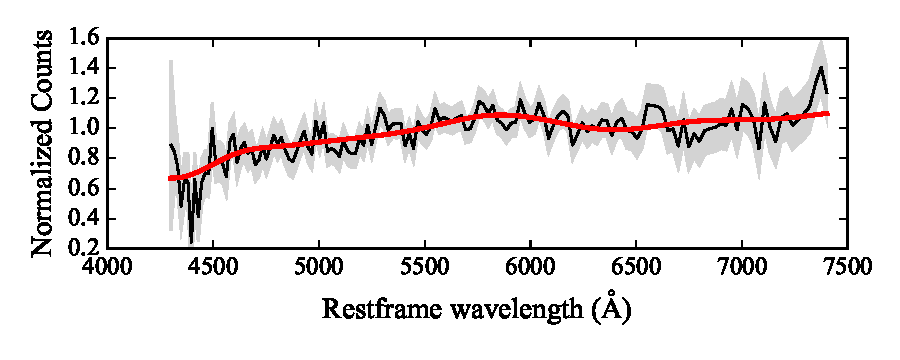
\includegraphics[width=1.0\columnwidth]{figs/knot1_pub_spec.pdf}
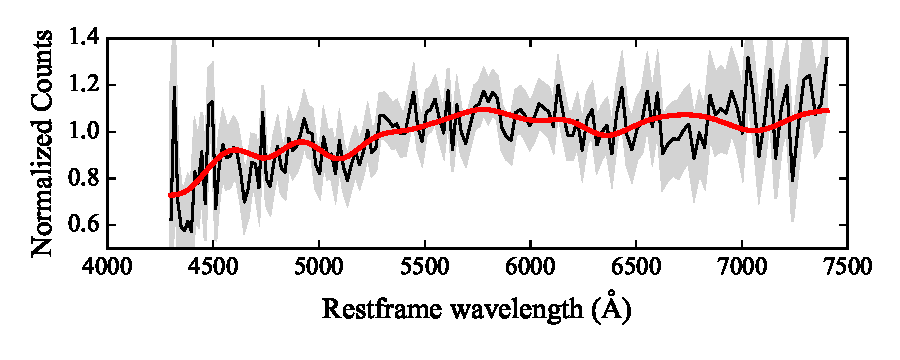
\includegraphics[width=1.0\columnwidth]{figs/knot2_pub_spec.pdf}
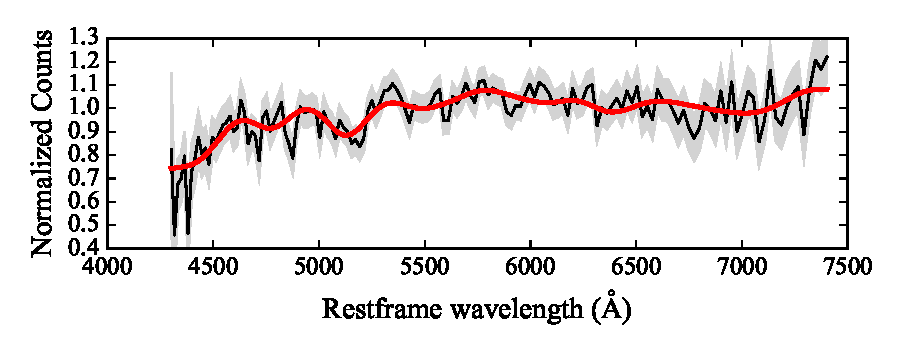
\includegraphics[width=1.0\columnwidth]{figs/knot3_pub_spec.pdf}
\end{center}
\caption{The normalized object spectra (black lines), the best fits (red lines), and the 68\% confidence intervals on the best fits (grey area) are shown for A2261 knots 1, 2, and 3 from top to bottom, respectively.}
\label{spectrafits}
\end{figure}

\subsection{Stellar Mass Estimates}

\fixme{Add text on SED fitting and provide stellar mass estimates here}

\section{Results}


\begin{figure}
\centering
%\vspace{3mm}
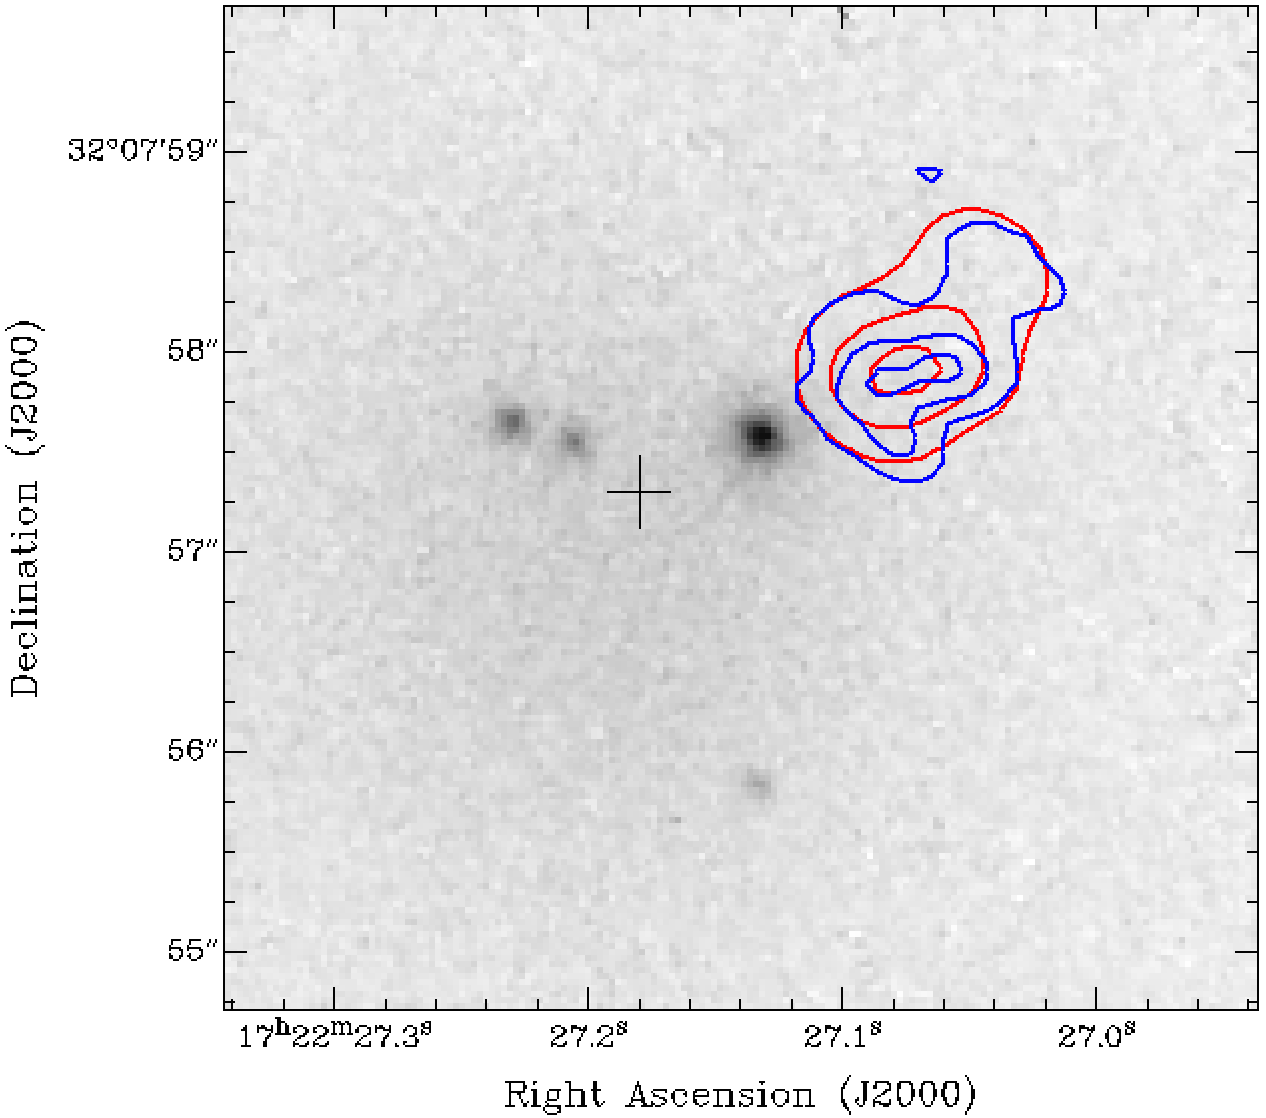
\includegraphics[width=0.95\columnwidth]{figs/contours+opt.png}
\caption{The 6\,GHz (red) and 10\,GHz (blue) contours overlaid on an image of the optical knots. Radio contours are at 30, 60, and 90\% of the respective image peaks.  The optical image is the CLASH HST F814W observation. \fixme{I don't like the placement of the cross, which is at the BCG photometric center not the core center. Perhaps both should be marked? Depends on discussion later.}}\label{fig:contopt}
\vspace{1mm}
\end{figure}




\begin{table*}
\centering
\caption{Astrometric Verification. Parenthesis indicate error on last digit.}
\begin{tabular}{llllll}
\hline
&\multicolumn{2}{c}{\bf Radio (J2000)}  &  \multicolumn{2}{c}{\bf Optical (J2000)}\\
{\bf Object} & {\bf R.A.}  & {\bf Dec} &  {\bf R.A.} &  {\bf Dec} & {\bf Offset ($''$)}\\
\hline
%Bright, resolved source to northwest (position of its non-extended/core component):
Dusty Spiral & 17:22:17.0107(8) & 32:09:12.7760(7) & 17:22:17.016(7)  & 32:09:13.1(1) & $0.09\pm0.14$ \\
Elliptical galaxy & 17:22:26.920(3) & 32:06:36.793(3) & 17:22:26.919(7) & 32:06:36.8(1) &  $0.02\pm0.15$ \\
%\hline
\src\ radio (10\,GHz)/optical core &17:22:27.072(3) & 32:07:57.8(2) & 17:22:27.190(7) & 32:07:56.8(1) & $1.80\pm0.25$\\
\hline
\end{tabular}\label{table:astrometry}
\end{table*}

\subsection{The radio source is offset from, but related to, \src's core.}
FIRST images originally indicated that there could be a radio component that is offset from the BCG's core. Our new higher-resolution images at 6 and 10\,GHz, shown in Figure \ref{fig:contopt}, confirm this offset. We find the radio centroid to be 1.8$''\pm0.25$ from the photometric center of the optical core.

To verify that an inaccurate radio/optical reference frame tie could not be not the cause of the offset, in our data we identified two field sources detected in both our VLA image and the SUBARU image. The positions of the optical centroid and the unresolved radio core component of these galaxies, and their radio/optical positional differences, are reported in Table \ref{table:astrometry}. The absolute astrometric offset of the reference sources is zero within error. In the same table we show the radio source's fitted position (fitting the X-band data for a single gaussian source), and the core's peak optical pixel location after the knots have been removed. We thus find the offset of the radio source to be significant and not due to a reference frame error.

We can also assess the probability that this radio source is a projected association and not a genuine one. The galaxy lies in the center of a dense cluster, thus general radio counts will likely underestimate this number. We thus measure the radio source count directly from the BCG2261 field using an image out to the full width half maximum image at C-band, which covers a FOV of 
% 4096 pixels at (0.101/3600) deg per pixel --> radius of circle = ((0.101/3600)*4096)/2 = 0.057 deg
% pi*0.057^2 = 0.0104 deg^2 field of view.
% 3 / 0.0104 = 288
% Poisson error on 3: (0.003 - 6.01) (0.0027 - 6.008)
% (0.27 - 601 per sq deg)
0.01\,deg$^2$ (wider than that of X-band). There were three objects in this field, including the offset central source under consideration, at or equal to the flux of the object in question within 1$\sigma$ flux errors. Thus, the count in this region is $R(>140\mu{\rm Jy})\simeq300\,{\rm deg}^{-2}$ in this field. The core of BCG2261, as given by the 3.2\,kpc (0.89$''$) cusp radius, covers $1.9\times10^{-7}\,{\rm deg}^2$. This means that a radio source of this flux density had a probability of $5.7\times10^{-5}$ to be in the galaxy core by chance; 
% This is very close to 4.0 sigma.
we are thus confident that the radio detection is related to the core.


\subsection{The radio source is a relic AGN component.}
Flux and extent measurements for the radio core are given in Table\,\ref{table:radio}. We can first explore the nature of this emission by noting its brightness temperature. 
% To make sure I do this right... https://science.nrao.edu/facilities/vla/proposing/TBconv
% 1.15740741e-7 is the source size assuming a 1 x 1.5 arcsecond object.
% C band: 1.36*(0.483)*(5104.58808)^2/(1.15740741e-7*4*ln(2)/pi)^2
% X band: 
% Redo this... 
% Use: http://www.atnf.csiro.au/people/Tobias.Westmeier/tools_hihelpers.php
% 1 x 1.5 arcsecond object
% Tb = 1.36 l^2 S / (src min x maj axis)
% With l in cm, S in mJy, arcsec for src size
% l = 5.104588 cm
% Tb = 1.36*(5.104588^2)*0.483/(1*1.5)
\fixme{This brightness temperature is orders of magnitude too high... recalculate it! Maybe it was a typo?}
Based on the integrated size and flux density measurements, we find a brightness temperatures at 6\,GHz of $T_{\rm B} = 1.64e+21$\,K. This brightness temperature, in addition to the high luminosities implied by the FIRST data ($\sim5\times10^23$\,W\,Hz$^{-1}$; \citealt{postman12}), indicate that this radio feature is AGN-related. The emission appears to cover a projected linear extent of around 3.5\,kpc, with a centroid offset of 6.5\,kpc from the core.
%and $T_{\rm B10} = !!!N$\,K at 6 and 10\,GHz, respectively. These values are sufficiently high to note that the source must be an 
The two-point spectral index measured by the VLA data finds an integrated spectral index of the source to be $\alpha=-2.1\pm0.2$, which is far steeper than the standard synchrotron spectra measured for radio emissions, which do show a broad range however are $\alpha\sim-0.7$ and usually $>-1.0$ for typical extended synchrotron jet features, and can have flat or positively sloped spectra for the core component that is most directly tied to the black hole engine \citep{ref,ref}. Figure \ref{fig:spix} shows a resolved two-point spectral index map of our 6 and 10\,GHz data across the full extent of the radio emission. It is clear from this map, albeit noisy, that there are no flat-spectrum sub-components in the observed emission that could feasibly represent an active core.

\begin{figure}
\centering
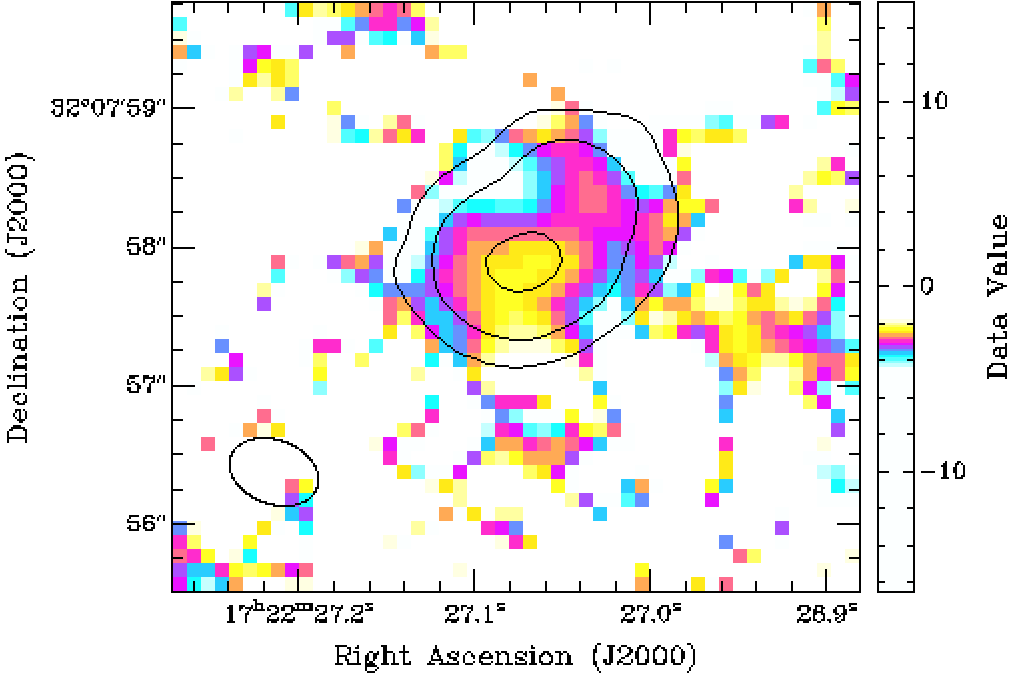
\includegraphics[trim=0mm 0cm 8mm 0mm,clip,width=0.95\columnwidth]{figs/spix.png}
\caption{\fixme{Need to make this graphic look better (i.e. make a 3sigma mask and do correct inner UV taper.} A spectral index map of the field, where spectral index $\alpha$ is defined as $S\propto f^{\alpha}$. Contours are shown for the tapered 6\,GHz data to give a reference for source placement. The lowest contour is at three times the root-mean-square noise in the 6\,GHz image; toward the edges of the object the contours become non-physical. The bulk of the source has a spectral index of just under $-2$, while its spectral index steepens somewhat towards the north-western spur. These indices are indicative of aging synchrotron emission, indicating a source that is not currently active. No core emission was detected to the 3$\sigma$ flux limit of 6.3\,$\mu$Jy and 3.6$\mu$Jy in the C- and X-bands, respectively.}\label{fig:spix}
\label{fig:last}
\vspace{1mm}
\end{figure}



\begin{figure}
\centering
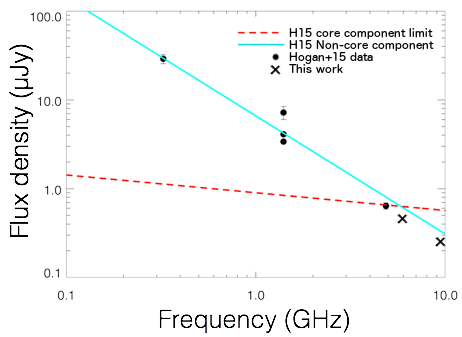
\includegraphics[width=0.95\columnwidth]{figs/spectrum-hoganplusus.png}
\caption{The radio spectral energy distribution of the \src\ radio emission. Our measurements indicate a consistency with a single power-law for low-frequency data, implying that a core component does not contribute significantly to this object. The steel spectral index of this object and the lack of core component implies that the radio jet source is in fact no longer active. \fixme{This plot needs to be way less ugly}}\label{fig:hoganspectrum}
\label{fig:last}
\vspace{1mm}
\end{figure}

Figure \ref{fig:hoganspectrum} shows the fitted low-frequency spectrum of \src\ from \citet{hogan+15} (hereafter H15), with our new higher-frequency data points points included. The H15 study aimed to perform core/non-core component modelling, and could only put a limit on the core emission from this source. Our data demonstrate that a single power-law model continues to fit this source across nearly two decades in frequency. Our 10\,GHz data point furthermore pushes the core component limit downward by a factor of $\sim$4, implying that the core contributes well under 1\,$\mu$Jy of flux density at GHz frequencies.  \fixme{I'd like to make a statement here about how this would be unexpected if such a whoppingly huge black hole in this galaxy were at all active. Need to figure out how to make that statement more quantitative, however.}

Based on the strict limits on core emission and the steep spectrum of the extended radio component, we conclude that this emission represents a fading jet component from a source that is no longer active. Such spectral steepening is expected from normal radiative aging of relativistic electrons in a synchrotron \citep{Scheuer+Williams1968}. This is exhibited by numerous radio galaxies, particularly at the broadest extent of their radio lobes, which are far enough from their energy source that their spectrum has begun to decay \citep{carilli+98}.


\fixme{Joe paragraph(s) here arguing briefly about how this is not a CSO.}


\subsection{How old is the radio relic?}
What is striking for this steep-spectrum radio source is that it has no core component, and is relatively compact. 
\fixme{Evolve the above points into a discussion of a limit on the radio lobe age depending on magnetic field strength; it must be very old because the bend frequency is well below 1\,GHz?!? This puts a limit on whether it might have been a recent merger that turned it off---although probably the only thing we can say is that it just marks when the thing ran out of fuel. So marks the ``at-least'' time for the last time the black hole ``ate something''. !!!}

%, and several views of the resulting images are shown in 
%Figs.\,\ref{fig:contopt}--\ref{fig:last}.

\subsection{The jet relic likely does not directly relate to the optical knots.}
While it is tempting to trace the jet axis's alignment back to \src's optical core position or perhaps knot 3, based on the likely age of the jet we conclude that the relative positioning of the radio and optical components cannot be meaningfully interpreted.
\fixme{leave it at that or is it worth getting into some ``sloshing'' discussion here as we have previously discussed?}
MENTION SLOSHING... it happens on the scale of a few crossing times which can be estimated and that number should be there.

%\noindent {\sc Main points to make here:}
%\begin{itemize}
%\item Discuss coincident field source positions (including a table) to demonstrate that {\bf the offset of the radio source is real}.
%\item {\bf Probabilistically, the radio source is associated with the BCG.} 
%\item Present Fig.\,\ref{fig:contopt} and a spectrum.
%\item Discuss brightnesses and compactness and make argument that {\bf this is certainly an AGN and not something else}
%\item The source is steep spectrum, and thus {\bf the jet is no longer active}.
%\item {\bf This is not a CSO.}
%\item Discuss morphology and alignment to the knots; does the jet originate in one of the knots? Basic answer we will conclude is: {\bf the morphology is sufficiently complex that we can't determine where the jet originated from. But, the evidence points to the fact that the jet is no longer active and thus was disrupted something like $10^6$ to $10^7$ years ago, otherwise we shouldn't be seeing this source at all, and with such a steep spectrum. Thus, the morphology is meaningless although might have some relevance to the discussions of sloshing (provide refs).}
%\item Put this radio source's properties in the context of other BCGs (i.e. Hogan et al 2015).
%\end{itemize}


\subsection{Knots 1 and 3 are, spectroscopically and photometrically, dwarf galaxies.}
\fixme{Kayhan/Marc/Leonidas section.} The point here is to present Kayhan's spectral fits for knots 1-3 and discuss why we think 1 and 3 are dwarf galaxies, however can't tell about what knot 2 is.

SHOW FIGURE: layered simulated super-massive black hole spectrum for knots 1 and/or 3 compared with the actual spectra, demonstrating the significant difference in velocity dispersion and that we basically rule out a massive black hole's presence in those knots.

NOTE: Bonfini\&Graham make the knots a little brighter than they were previously. Are they something that was bright and have been truncated? These all need to be discussed together. We should line up the arguments and note if these things are morphologically unusual. Now that this has been contested we need to tighten the screws on this source.

Marc: ``when we did our photometric model to knot 3 there is a small residual to the northwest which Graham is presumably calling the 5th knot. There's also an underlying larger, diffuse feature to the south of knot 3 and we're not sure what to make of that.'' Tod: ``this whole core thing is sloshing around so hard to interpret.''

\subsection{\fixme{Is Knot 4 a Stellar Shroud?}}
Figure\,\ref{fig:knotSEDs} shows the optical spectral energy distirbutions for knots 1--4 from the archival imaging data. The dashed red SED is that for the BCG (renormalized to match each knot?s flux in the F814W band). The difference plots at the bottom of each SED plot are the knot ABmag minus that for the renormalized BCG ABmag. Any positive slope in that difference suggests knot is a bit bluer than the BCG. Negative slope indicates knot is redder than BCG. Knots 3 and 4 exhibit a bluer color than the \src\ galaxy itself, implying a separate stellar population.

From telecon: It's intriguing but not conclusive; nuclear clusters can be a slightly different color than the host so if the black hole only dragged the nuclear cluster it might be slightly bluer. However, it does seem there's disagreement in the stellar populations between the BCG core and knot 4.

\fixme{THIS ASPECT NEEDS TO BE DISCUSSED!!!}

\fixme{\subsection{Sarah's optical analysis section notes}
\noindent Important to include here:
\begin{itemize}
\item Predictions already done for the proposal on how well we would have detected a $10^9\,\msun$ black hole in the knots (perhaps show the graphic if appropriate?).
\item Description of fitting procedure, if it's not already in Sec.\,\ref{sec:HSTdata}
\item Presentation of results for knots 1--3 and confidence in the fitting results.
\item {\bf Knots 1 and 3 are dwarf galaxies}
\item {\bf Assessment of knot 2: basically both dwarf galaxy and SMBH are supported (i.e. we don't have sufficient S/N).}
\item Include a note on the fact that STIS was less sensitive than expected?
\end{itemize}}
%\subsection{Optical-Radio Reference Frame Tie}
%{\sc We double checked the reference frame with 2-3 stars detected by HST and VLA blah blah blah.} 


%\begin{figure}
%\vspace{10mm}\centering
%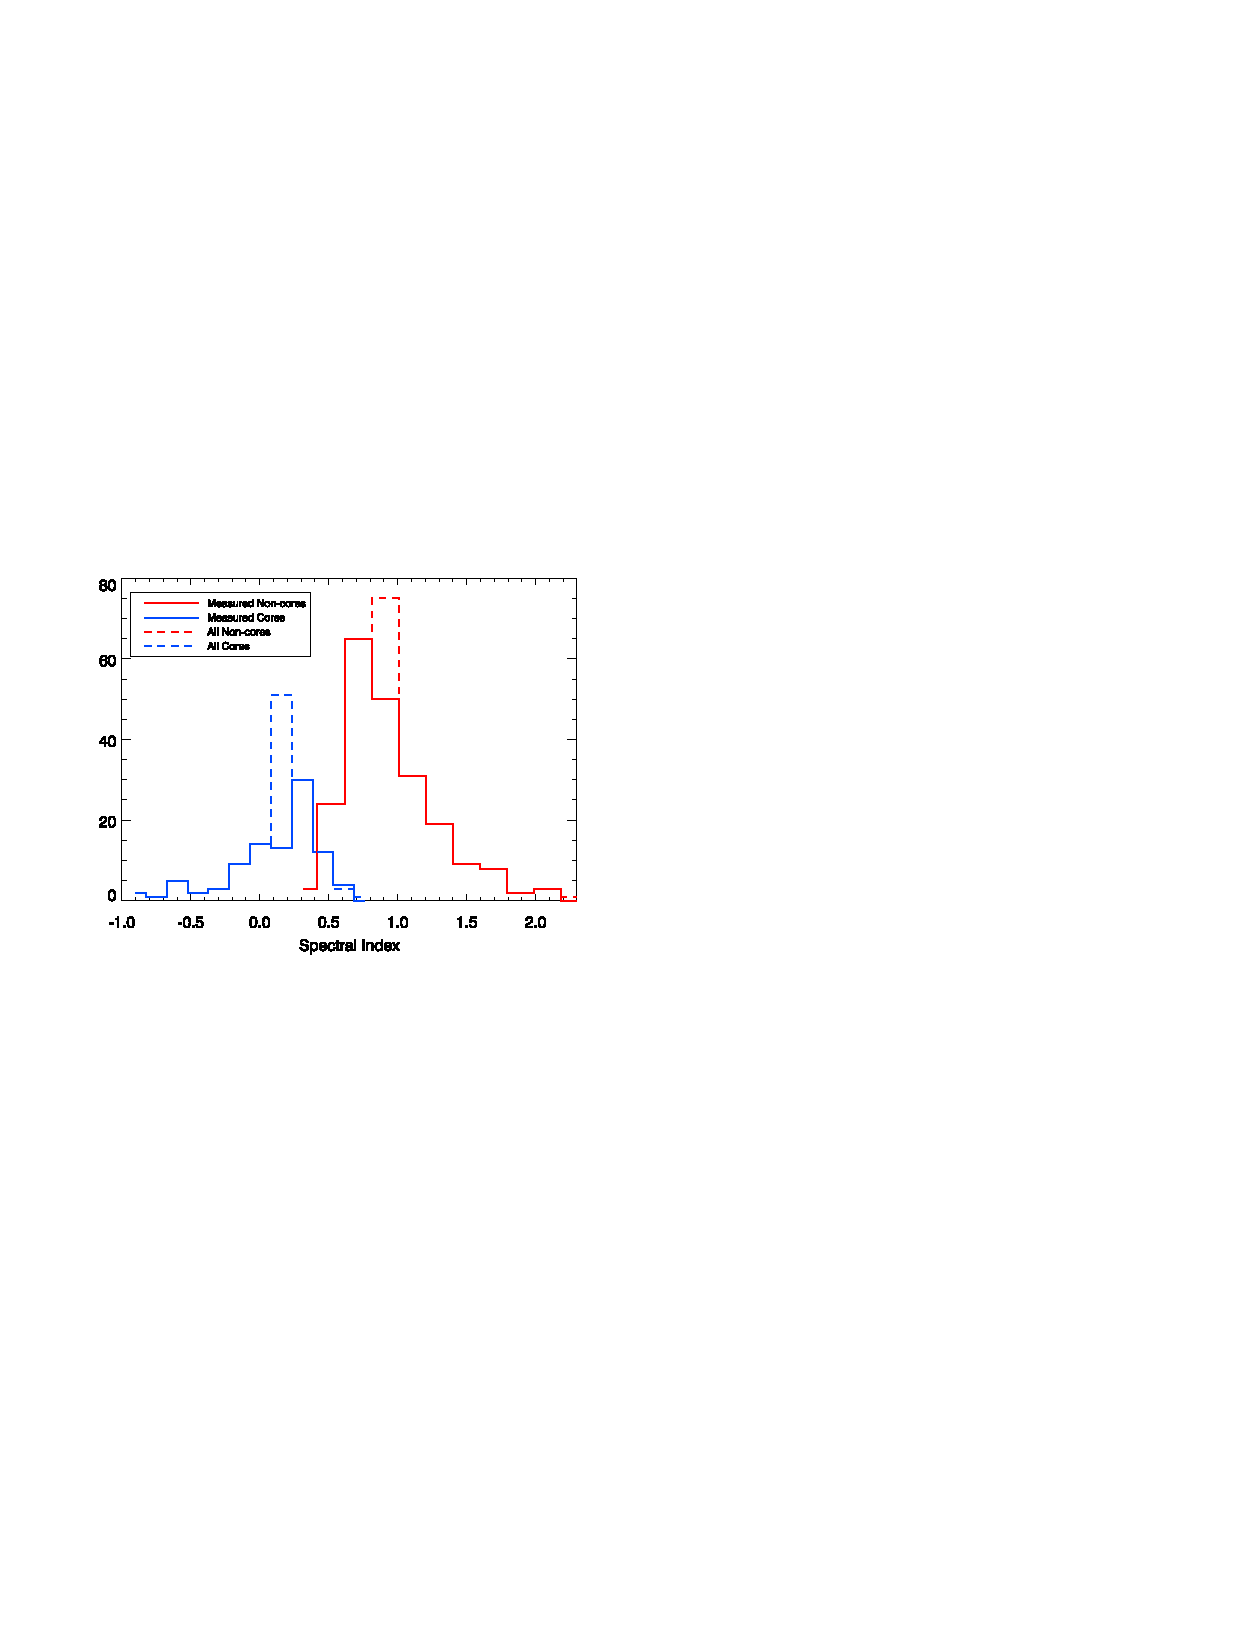
\includegraphics[width=0.95\columnwidth]{figs/bcg-spixes.pdf}
%\caption{The spectral index distribution of the BCGs in \citet{hogan+15}.}\label{fig:BCGspixdist}
%\vspace{1mm}
%\end{figure}


\section{Discussion}

\subsection{What happened to \src's gigantic black hole?}
Include here a discussion of the possible things that might have happened to the radio jet. We basically know that it was on sometime in the last billion years or so, but within the last $\sim$$10^7$ years it lost its fuelling source. 

Potential \src\ radio source histories based on this:
\begin{itemize}
\item The jet was on before the binary's coalescence. The coalescence shut it off. That allows us to date the coalescence time, and make interesting statements about how long cores stay around, how far the BH could have travelled if recoiling, whether knots 2 and 4 remain viable candidates based on that analysis, and whether the recoil would have been large enough and have been going on long enough to actually do what Postman+12 said it could do to the core.
\item The jet turned on after the binary's coalescence but then ran out of fuel because it was recoiling. This relates to AGN lifetimes within a recoil, and we can under this hypothesis set limits on how long the thing could have been recoiling based on Blecha et al.-type analyses. We can then do similar assessments as to the previous point; the timescales here would be a bit longer.
\item The jet was triggered by infall of gas from a smaller galaxy, not necessarily a major merger... this seems a realistic possibility given the at least two dwarf galaxies that are floating around the core. In this case, we don't necessarily need a big coalescence or recoil to have happened anytime recently. I'm not sure what more we could say about the implications of this possibility but certainly my co-authors might have thoughts on how this point could be further assessed with other information/data we have.
\end{itemize}

These hypotheses should all be perhaps weighed against one another using previous conclusions from Postman et al. (2012).

\subsection{Dynamics and properties of the knots}
Discuss what is happening to knots 1 and 3; that is, they are still well within the escape velocity of the BCG and are likely being cannibalized by the galaxy. This is fairly unsurprising given that this is a big busy cluster. Make some dismissive statement about why they are both blueshifted at fairly high velocity (i.e. they're still falling into it, we just happen to be seeing them on a path towards us).

\subsection{Other possibilities for this system}
Include a discussion of Graham et al 2016, https://arxiv.org/abs/1610.00801

\subsection{How atypical are the radio properties of \src?}
\fixme{I'm considering a section comparing this object to the other general radio properties of BCGs. However, that data is pretty scattered and this discussion appears it will likely simply amount to ``\src's radio emission is atypical of BCGs because it's steeper and more compact that most others''. Below is my cursory look at this. Is it worth including?}

{\bf Luminosity distribution:} \citet{hogan+15} provides BCG radio luminosity functions for galaxies at 1.4\,GHz. Archival VLA data provides a 1.4\,GHz flux of \mbox{$S_{\rm 1GHz} = 3.1$}\,mJy and so \mbox{$L_{\rm 1GHz}\simeq3\times10^{22}~{\rm W~Hz^{-1}}$} given \src's redshift $z=0.224$. According to the Hogan et al.\ luminosity measurements, \src\ is typical of 80--90\% of BCG luminosities.

{\bf Spectral index properties:} \src\ appears to be abnormal among BCG spectral indices; its spectrum is much steeper than any of the objects shown in the distribution reproduced in Fig.\ \ref{fig:BCGspixdist}. 
%It is possible we need to improve our u,v coverage or improve the tapering scheme for comparative imaging to improve our spectral index measurements. 
%This is being investigated.

%\item 
{\bf Morphologies/ages:} It appears unusual to be so small. Things without (spectroscopically-identified) cores are fairly common---but that doesn't mean they don't morphologically have a core. 
%\item {\bf Physical offsets: any others?} 
%\item {\bf Image catalog.} 
%\end{itemize}


\fixme{BASIC HEADLINE SUGGESTED BY TOD: ``We selected this galaxy based on its extreme optical photometric properties, and it ended up having equally unusual radio properties.''}

\subsection{Other points of discussion?}

\subsection{Prospects for further exploration}
A2261 has two \emph{Chandra} exposures of 10 and 25 ksec (ObsIDs 550 and 5007, respectively), which do not conclusively reveal any accretion onto a SMBH.  The X-ray flux is those data is dominated by 0.5--2\,keV emission from hot cluster gas, showing a cooled core \citep{2005MNRAS.359.1481B}.  Above 2\
,keV, there are is some emission, possibly a point source consistent with knot 4, though it is far too faint to reliably distinguish it from cluster gas emission.  Deeper \emph{Chandra} observations can better reveal low-level accretion onto a SMBH and has the angular resolution to localize a point source such that it can be determined whether it is in one of the knots or at the core photometric center.  For example, if the black hole has a mass of $10^{10}\,\msun$, and it is emitting in the 2--7\,kEv band at an Eddington fraction of $10^{-6}$ as a power-law with photon index $\Gamma = 1.9$, a 100 ksec observation would detect 5 photons in the band, sufficient for significant detection above the background.  Such an observation would also be sensitive to a bow shock created by a recoiling SMBH and thus could provide strong positive evidence if it exists.

Maybe just put this section in as part of the conclusions. The idea is to must on what further studies could be done of this galaxy.

%^&\section{Is the black hole recoiling?}
%^&Here we lay out the major pieces of evidence, external to the work presented here, for a SMBH recoil in this galaxy:
%^&\begin{itemize}
%^&\item Big core (dynamical process).
%^&\item Offset core (recent disturbance).
%^&\item Lack of cusp but should have massive SMBH.
%^&\end{itemize}

%
%\begin{figure*}
%\centering
%\includegraphics[width=0.97\columnwidth]{cband.png}~~~~~
%\includegraphics[width=0.95\columnwidth]{xband.png}
%\caption{\emph{Left:} The 6\,GHz contours and image. Contours are at 3, 4, 8, 16, 32, and 64 times the root-mean-squared image noise. \emph{Right:} The 10\,GHz contours and image. Contours are at 3, 4, 8, and 16 times the root-mean-squared image noise.}\label{fig:6and10}
%\end{figure*}


%^&\begin{figure}
%^&\centering
%^&\includegraphics[width=0.9\columnwidth]{cband.png}
%^&\caption{The 6\,GHz contours and image. Contours are at 3, 4, 8, 16, 32, and 64 times the root-mean-squared image noise.}\label{fig:contopt}
%^&\end{figure}
%^&
%^&\begin{figure}
%^&\centering
%^&\includegraphics[width=0.9\columnwidth]{xband.png}
%^&\caption{The 10\,GHz contours and image. Contours are at 3, 4, 8, and 16 times the root-mean-squared image noise.}%^&\label{fig:contopt}
%^&\end{figure}

%\begin{figure*}
%\centering
%\includegraphics[width=0.98\columnwidth]{c-gray-optoverlay.png}~~~~~~
%\includegraphics[width=0.92\columnwidth]{x-gray-optoverlay.png}
%\caption{The optical component locations overlaid on the 6\,GHz data (left) and the 10\,GHz data (right).}\label{fig:6and10opt}
%\end{figure*}



%^&\begin{figure*}
%^&\centering
%^&\subfigure[]{
%^&%\includegraphics[width=0.7\textwidth,angle=270,trim=0mm 0mm 0mm 2mm, clip]{figs/blah.ps}
%^&}\\
%^&\subfigure[]{
%^&%\includegraphics[width=0.43\textwidth,trim=0mm 0mm 0mm 0mm, clip]{figs/}
%^&}\quad
%^&\subfigure[]{
%^&%\includegraphics[width=0.43\textwidth,trim=0mm 0mm 0mm 0mm, clip]{figs/}
%^&}
%^&\caption{}\label{fig:plots}
%^&\end{figure*}

\section{Conclusions}
The radio jet does not necessarily favor a recoil, but is certainly supportive of that hypothesis. But if there was a recoil that created the offset jet that we observe, then we infer that X Y and Z must be true.

\fixme{Under all scenarios, knot 2 still remains the only(?) viable candidate for a recoiling SMBH host.}

\section{Acknowledgements}
The National Radio Astronomy Observatory is a facility of the National Science Foundation operated under cooperative agreement by Associated Universities, Inc.
Part of this research was carried out at the Jet Propulsion Laboratory, California Institute of Technology, under a contract with the National Aeronautics and Space Administration.


%\section{A bit of extra text to scrap thru when filling in the paper...}
%\subsection{Astrometry}
%To provide a sufficiently accurate reference tie, we sought at least two unresolved radio reference sources that were coincident with optical objects within this field of view. Our full-resolution VLA observations (not averaged in time or frequency) allow for full imaging of this field of view without distortion arising from bandwidth- and time-smearing effects.

%\subsection{Spectral index}
%Using the integrated flux, the net two-point spectral index between 6 and 10\,GHz is $\alpha=-2.56$.


%\subsection{Radio properties of BCGs}
%Placing the radio emission from \src\ in context requires the examination of the radio properties of other BCGs. The study of \citet{hogan+15} provides a thorough examination of this. 


\subsection{Other papers maybe of relevance}
Major dry mergers in BCGs\\
http://adsabs.harvard.edu/abs/2009MNRAS.396.2003L

A recent study on spectral aging in case we feel the need to (badly) estimate an age of the radio emission\\
http://adsabs.harvard.edu/abs/2013MNRAS.435.3353H

``Core sloshing,'' maybe, in a BCG leading to peculiar radio emission\\
http://www.aanda.org/articles/aa/pdf/2013/10/aa22023-13.pdf

\bibliographystyle{mn2e}
\bibliography{abel}

\end{document}